%!TEX encoding = IsoLatin

%
% Chapitre "Concept retenu"
%

\chapter{Concept retenu}
\label{s:concept_retenu}

\section{Matrice de décision}

La matrice de décision du projet Fish \& Chips est présentée à la table \ref{t:matrice_decision}. Elle permet d'illustrer clairement le taux de satisfaction de tous les critères pour chaque concept afin de faire un choix éclairé. Les barèmes sont basés sur les critères du tableau \ref{t:criteres} et les pondérations sont ajustées de manière à bien refléter l'importance de chaque besoin du projet. 

\begin{table}[htp]
   \footnotesize
   \centering
   \scalebox{1.0}{
   \begin{tabular}{|c|c||c|c|c|c|}
        \hline
        Critère d'évaluation & Pond. & Concept 1 & Concept 2 & Concept 3 & Concept 4\\
        \hline
        \hline
        \textbf{Qualité du produit} & \textbf{65\%} &\textbf{ \%} &\textbf{ \%} &\textbf{ \%} &\textbf{ \%}\\
        \hline
        Résolution du capteur & 10\% & 4,9 & 8 & 3,3 & 2,4 \\
        Identification des poissons & 10\% & 9,9 & 9,9 & 9,9 & 9,9 \\
        Volume d'analyse & 5\% & 1,2 & 1,2 & 4,9 & 3,5 \\
        Capacité de stockage des données 
        & 5\% & 5 & 0,4 & 4 & 5 \\
        Durée de vie de l'alimentation du système & 5\% & 1,3 & 5 & 3,5 & 3 \\
        Acheminement des informations & 5\% & 4 & 0,5 & 3,2 & 2\\
        Fiabilité du système de sécurité & 5\% & 4,4 & 4,4 & 4,4 &  4,3 \\
        Résistance à la profondeur & 4\% & 0,6 & 0,6 & 0,5 & 2\\
        Taille des spécimens observés & 4\% & 3,7 & 3,6 & 4 & 3,4\\
        Nombre de fonctionnalités de l'alarme & 4\% & 0,9 & 0,4 & 4 & 0,4\\
        Puissance de calcul & 4\% & 3,1 & 1,3 & 1,3 & 1,3 \\
        Utilisation de l'interface graphique & 4\% & 4 & 3,2 & 1,6 & 2,4\\
        \hline\hline
        \textbf{Performance} & \textbf{20\%} & \textbf{ \%}  &\textbf{ \%} &\textbf{ \%} &\textbf{ \%} \\
        \hline
        Précision du logiciel de reconnaissance & 15\% & 13,6 & 14,3 & 5,5 & 3,6 \\
        Précision de la régulation & 2\% & 2 & 1,9 & 0,4 & 2 \\
        Précision de la mesure de température & 2\% & 2 & 1,9 & 0,4 & 1,98 \\
        Précision de la mesure du temps & 1\% & 1 & 1 & 1 & 1 \\
        \hline\hline
        \textbf{Coûts} & \textbf{15\%} &\textbf{ \%} & \textbf{ \%}& \textbf{ \%}&\textbf{ \%} \\
        \hline
        Coût de main d'oeuvre & 12\% & 0 & 0 & 1,4 & 0,9 \\
        Coûts du matériel & 3\% & 2,4 & 2,2 & 2,4 & 2,57\\
        \hline\hline
        \textbf{Total} & \textbf{100\%} &\textbf{64.0\%} &\textbf{59,8\%} &\textbf{ 55,7\%} &\textbf{51,65\%} \\
        \hline
   \end{tabular}}
    \caption{Matrice de décision du projet Fish \& Chips}
    \label{t:matrice_decision}
\end{table}




\section{Analyse de la matrice de décision}

Avec un taux de satisfaction de xx \%, c'est le concept 2 qui est le mieux adapté aux besoins du projet. Il se démarque surtout par (insérer critère) qui a une plus grande pondération et donc une plus grande importance dans le projet. Les concepts xx, xx et xx ont respectivement des taux de satisfaction de xx\%, xx\% et xx\%. Ils ont surtout des lacunes au niveau de blablabla critères. Le concept 2 est donc retenu et fait l'objet d'une analyse plus détaillée en \ref{ch7:concept_retenu}.

\section{Description du concept retenu}
\label{ch7:concept_retenu}

\textbf{Prise de mesure}
\begin{itemize}
    \item Caméra (OV5640)
    \item Mesure température (thermistance)
    \item Date et heure
\end{itemize}

\textbf{Support physique}
\begin{itemize}
    \item Hardware pour runner le code (PC Custom)
    \item Batterie (rechargeable le best svp)
    \item Régulation (Peltier)
    \item Stockage de données (Carte SD)
    \item Acheminement des infos (Manuel)
\end{itemize}

\textbf{Logique de programmation (renommer)}
\begin{itemize}
    \item Identification (Neurones)
    \item Sécurité (p-e dans comm., encryption?)
\end{itemize}

\textbf{Communication}
\begin{itemize}
    \item Interface graphique (lequel)
    \item Sécurité ??
    \item Envoi de l'alarme (srm Amazon)
\end{itemize}

\clearpage

\subsection{Prise de mesure}
Dans l'optique de la prise des mesures sous l'eau, on utilisera le capteur OV 5640. Ce capteur d'image n'est pas celui avec la meilleure résolution. Cependant, la caméra rempli tout à fait les exigences du client. Son grand intérêt vient du fait qu'elle soit programmable via USB et qu'elle soit diaponible à un faible coût (60\$) pour un temps de livraison réduit et sa taille et son poids réduits. De ce fait, ce capteur semble le meilleur pour notre système. 


Pour mesurer la température à l'intérieur et à l'extérieur de la machine, on utilise un Raspberry Pi connecté à une thermistance. Cet assemblage rudimentaire permet de mesurer à peu de frais avec une grande précision les températures que le client souhaite connaître. L'avantage d'un module programmable tel que celui ci est qu'il est ensuite plus facile d'implémenter une régulation de la température, ici effectuée avec le module Peltier. Cette partie du système se procure très facilement pour un prix d'une vingtaine de dollars.


De plus, afin de déterminer les moments où les images sont prises, on utilise un module de type datetime. Grâce à ce concept de programmation, on pourra facilement savoir à quels moments quelles images ont été prises. Cet outil est très intéressant dû au fait qu'il soit précis à la seconde près et soit totalement gratuit pour connaître les images.

\subsection{Support physique}
Ensuite, pour supporter et analyser les données disponibles, on utilisera le matériel informatique disponible dans l'ordinateur personnalisé. Grâce à cet ordinateur, le code pourra être exécuter. Ensuite, grâce au code, toutes les informations seront traitées et organisées de façon à satisfaire les exigences du client.

De plus, par l'alimentation avec les batteries rechargeables Energizer, il sera possible de fournir à notre machine une puissance électrique tout à fait suffisante pour alimenter le capteur et assurer son fonctionnement sur une durée de 2 semaines. De plus, comme elles sont rechargeables, il est possible de ne pas avoir à en racheter d'autres sur la durée de l'utilisation du capteur.

Comme le système consommera de la puissance électrique, la machine aura besoin d'un système de refroidissement pour dégager la chaleur et empêcher le système de surchauffer, ce qui pourrait endommager la machine et causer des problèmes lors de la prise des mesures. À cet effet, nous utiliserons des modules Peltier tel que mentionné précédemment. Modèles pourront facilement être contrôlés grâce au Raspberry ¨Pi qui pourra assurer l'équilibre de la température dans la machine.

Afin de stocker toutes les données qui seront accumulées tout au long de la durée d'utilisation de la machine, nous utiliserons le disque SSD de Kingston d'une capacité de stockage de 240 Go. Cette capacité de stockage a été jugée comme suffisante lors de l'étude préliminaire. Pour contenir ces données sur une durée estimée de deux ans, nous pourrons sauvegarder toutes les données tel que souhaité par le client.

Enfin, pour acheminer les informations, cela sera fait de façon manuelle: lorsque le capteur sera retiré au bout de 14 jours, il sera possible de retirer les données capturer par le Raspberry Pi et de les stockées sur le disque SSD. Ce système nous permettra de sauvegarder les données sur le SSD pendant que la carte SD du Raspberry Pi continuera de capturer les nouvelles données.

\subsection{Logique de programmation}

Lors de la capture des images, il a été exigées par le client de déterminer de quels poissons il s'agissait sur l'image. Pour accomplir cette mission, il a été décidé d'utiliser un réseau de neurones convolutionnel avec la librairie Tensorflow. Ces outils informatique entraînés à l'identification des poissons du Québec pourront, dès l'image capturée, déterminer l'espèce du poisson et le tout pourra être stocker avec le disque SSD.

Pour sécuriser les données acquises par le capteur, un système d'encryption des données a été choisi

\subsection{Communication}


\section{Conclusion}

lets fucking gooooooooooo

\begin{figure}
    \centering
    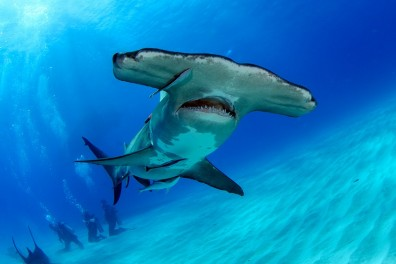
\includegraphics[width=\linewidth]{fig/requinmarto.jpg}
    \caption{Diagramme physique de la solution retenue pour le projet Fish \& Chips}
    \label{fig:concept_retenu}
\end{figure}

